\documentclass[10pt,a4paper]{article}
\usepackage[margin=.76in]{geometry}\usepackage[T1]{fontenc}
\usepackage{lmodern,microtype,booktabs,graphicx,xcolor,hyperref}
\hypersetup{hidelinks}\setlength{\parindent}{0pt}\setlength{\parskip}{6pt}\emergencystretch=3em
\title{IDM-Viz: Seed-Held-Out Forecast of Future Harm}
\author{Ahmed Bilal (23I-2581) \and Umar Behram (23I-2604)}\date{16 November 2026}
\begin{document}\maketitle
\begin{abstract}
We tested a locked pooled logistic model for whether mean accuracy across the next five complete synthetic monitoring batches falls more than five percentage points below that stream's historical reference. Thirty development and thirty disjoint evaluation seeds span seven known generator conditions and delays 0, 5 and 20. The model using released-label history is compared with time-only and currently available unlabeled-monitor predictors. This evaluates interpolation within known synthetic laws, not transfer to unseen regimes or real streams.
\end{abstract}
\section{Protocol}
Forecasts are issued at batch t for batches t+1 through t+5; t=1,...,19. A monitoring label is available only when its batch plus delay is strictly less than t; same-clock labels arrive after the forecast. Three StandardScaler plus LogisticRegression(C=1) models are trained only on 30 development seeds. No seed or condition identifiers enter predictors and no threshold was tuned. The evaluation unit for uncertainty is the held-out seed, not the repeated row. Two thousand paired whole-seed bootstrap replicates compare Brier scores.
\section{Results}
\begin{table}[ht]\centering\small\begin{tabular}{lrrrr}\toprule Predictor set & ROC AUC & AP & Brier & Log loss \\\midrule
time only & 0.640 & 0.483 & 0.231 & 0.650 \\
unlabeled monitor & 0.838 & 0.760 & 0.166 & 0.484 \\
full released & 0.865 & 0.818 & 0.149 & 0.446 \\
development prevalence$^*$ & 0.500 & 0.418 & 0.243 & 0.680 \\
last released harm$^*$ & 0.639 & 0.573 & 0.258 & 3.114 \\
current concern$^*$ & 0.650 & 0.632 & 0.327 & 1.960 \\
\bottomrule\end{tabular}\caption{Pooled held-out performance over 11,970 future-window forecasts per predictor (30 seeds x 7 conditions x 3 delays x 19 origins). $^*$Heuristic score comparators; current concern is not trained or calibrated as a future-risk probability.} \end{table}
\begin{figure}[ht]\centering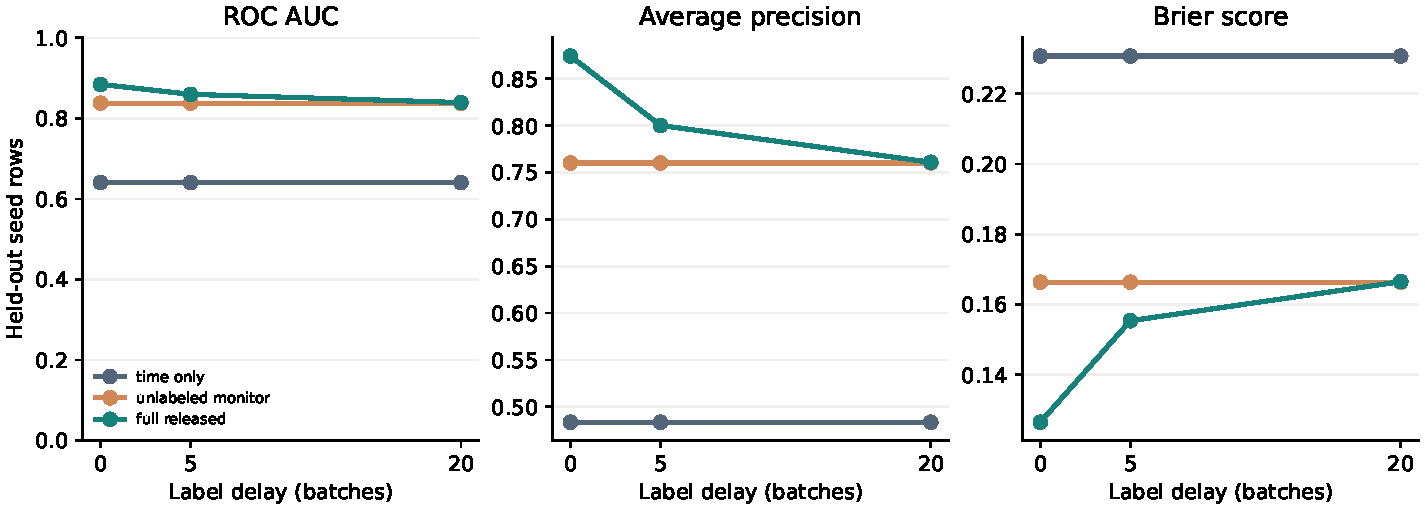
\includegraphics[width=.98\linewidth]{forecast_metrics.pdf}\caption{Discrimination and probability error by label delay. AP should be interpreted against the held-out target prevalence.}\end{figure}
Paired seed-bootstrap Brier differences (first model minus second; negative favors the first) were: time only minus unlabeled monitor Brier: +0.0644 [+0.0603, +0.0674]; unlabeled monitor minus full released Brier: +0.0169 [+0.0160, +0.0179]; time only minus full released Brier: +0.0813 [+0.0776, +0.0839]. The bootstrap resamples 30 seeds as clusters and retains each seed's seven conditions and three delays together.
\section{Interpretation and limitations}
This experiment directly evaluates a prospective five-batch outcome using only information available at forecast time. It does not establish that alarms cause harm, that a forecast is useful to an analyst, or that performance transfers beyond these seven synthetic mechanisms. The seven conditions are known during development, and the pooled model can exploit time-dependent prevalence; the held-out seeds are independent draws under those same laws. The synthetic labels share the generator construction, so this is not external validation. Small held-out seed count leaves material uncertainty. No calibrated risk certificate or intervention benefit is claimed. The online feature artifact excludes correctness and harm labels; future targets are stored separately for evaluation.
\section{Reproduction}
\begin{verbatim}
python scripts/run_future_harm_forecast.py
python scripts/evaluate_future_harm_forecast.py results/phase3/future_harm_forecast_20261116_v1
python scripts/report_future_harm_forecast.py
\end{verbatim}
The protocol lock, split, saved probabilities, evaluator targets, metrics and paired bootstrap are included with the editable \TeX source.
\end{document}
